\section{平面与平面系统}
\begin{definition}[平面光学元件]
    工作面为平面的光学元件,对物体没有放大和缩小的功能,分为平面折射和反射原件。
    \end{definition}
其可以
\begin{itemize}[nosep]
\item 改变光轴位置和方向
\item 改变像的坐标
\item 折叠光路,减小形体和质量
\item 分光
\item 测量,扩大系统观察范围
\end{itemize}
\subsection{平面镜}
平面反射镜,简称平面镜,\textbf{唯一成完善像元件}(理想成像)。
对于平面镜,常见性质为
\begin{align}
    r=\mathbf{-}\infty &\hspace{0.3cm}   n'=-n\tag{4.1.1.a}\\
    \beta=1& \hspace{0.3cm} l'=l \tag{4.1.1.b}\\
   y=y'& \tag{4.1.1.c}
\end{align}
\begin{description}[leftmargin=0.9cm,style=nextline,nosep]% nosep没有垂直间隔
    \item[镜像]  左右手坐标系颠倒。
    \item[$2\alpha$] 平面镜旋转$\alpha$,反射光线同方向旋转$2\alpha$
\end{description}
        \begin{figure}[H]
            \centering
            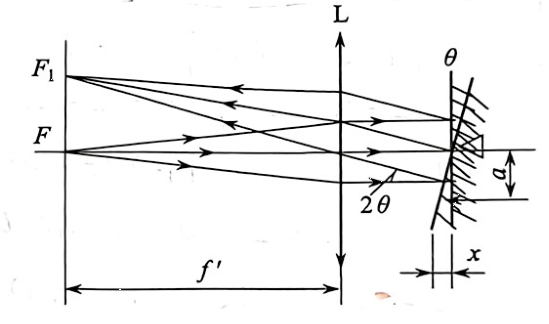
\includegraphics[width=7cm]{img/4.2.png}
            \end{figure}
$2\alpha$ 性质常被用于测量,如上图2所示,有
\begin{align}
    FF_1=2f'\theta \tag{4.1.2.a}\\
    FF_1=2f(\frac{a}{x}) \tag{4.1.2.b}
\end{align}
\subsubsection{双平面成像}
        \begin{figure}[H]
            \centering
            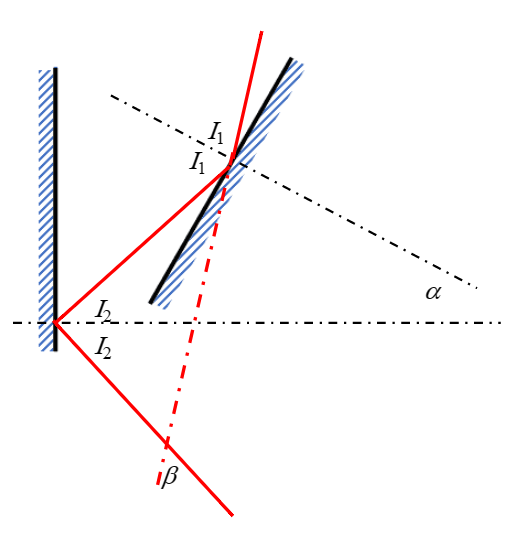
\includegraphics[width=5cm]{img/4.3.png}
            \end{figure}
出射光线与入射光线夹角只与平面镜二面角有关。设入射光线和出射光线单位向量分别为$\vec{r_{in}},\vec{r_{out}}$,第一个和第二个镜面单位法向量为(入射到的第一个)$\vec{n_1,\vec{v_2}}$。有
\begin{equation}
\frac{\cos <\vec{r_{in}},\vec{r_{out}}>}{\cos <\vec{n_1},\vec{n_2}>}=2\tag{4.1.3}
\end{equation}
\subsection{平行平板}
        \begin{figure}[H]
            \centering
            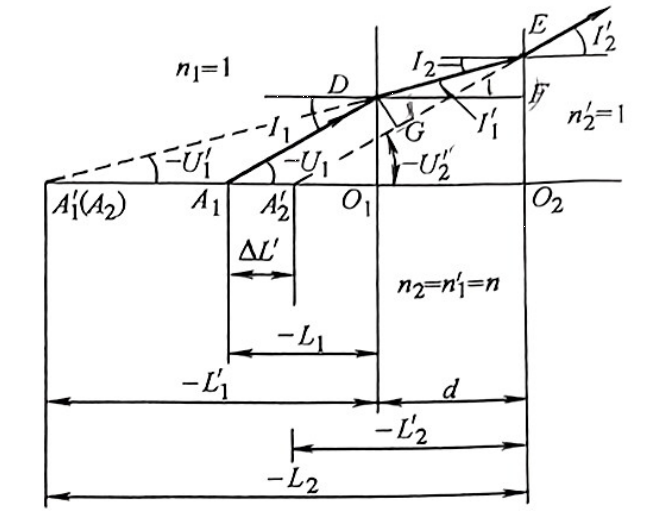
\includegraphics[width=6cm]{img/4.4.png}
        \end{figure}
\begin{equation}
\begin{aligned}
    \Delta T=DG&=\frac{DE}{\sin(I_1-I_1')} \\
    &=\frac{d}{\cos I_1'}\sin(I_1-I_1')\\
    &=\frac{d}{\cos I_1'}(\sin I_1\cos I_1'-\cos I_1\sin I_1')\\
    &=\frac{d}{\cos I_1'}[\sin I_1'(n \cos I_1'-\cos I_1)]\\
    &=d\sin I(1-\frac{\cos I_1}{n \cos I_1'})\\
    &=d\sin I(1-\frac{\tan I_1}{\tan I_1'})
    % &(n\sinI=n'\sinI')
\end{aligned}\tag{4.2.1}
\end{equation}

\begin{align}
\Delta L'&=\frac{DG}{\sin I_1} \tag{4.2.2.a}\\
&=d(1-\frac{\cos I_1}{n \cos I_1'})\tag{4.2.2.b}\\
&=d(1-\frac{\tan I_1}{\tan I_1'}) \tag{4.2.2.c}
\end{align}

显然,其不能成完善像。一些常见的符号含义
\begin{align}
    L_1=H_1A_1 &\hspace{0.3cm}   L_1'=H_1'A_1'\tag{4.2.3.a}\\
    L_2=H_1A_2 &\hspace{0.3cm}   L_2'=H_1'A_2'\tag{4.2.3.b}\\
   d=H_1H_1'& \hspace{0.3cm} \Delta L'=A_1 A_2' \tag{4.2.3.c}
\end{align}
显然
\begin{equation}
L_2'=-d+L_1+\Delta L'\tag{4.2.4}
\end{equation}
或者
\begin{equation}
\Delta L'=A_1A_2'=-L_1+d+L_2'\tag{4.2.5}
    \end{equation}

    \subsubsection{近轴区等效}
    \begin{equation}
    \Delta L'=d(1-\frac{1}{n}) \tag{4.2.6}
    \end{equation}
    等效空气平板
    \begin{equation}
    \overline{d}=d-\Delta L'=\frac{d}{n}\tag{4.2.7}
    \end{equation}
    轴向位移如下,换小写就行。
    \begin{quote}
    {\qquad\parindent2\ccwd\kaishu\zihao{5}
    所谓等效:
是指同一入射光线,在入射面的
投射高度相同,在出射面的投射
高度也相同;
    }
    \end{quote}
\subsection{反射棱镜}
\begin{description}[leftmargin=1.7cm,style=nextline,nosep]% nosep没有垂直间隔
    \item[光轴] 光学系统中的光轴在棱镜中的部分。
    \item[入射面和出射面] 
    \item[棱线] 工作面之间的郊交线  
    \item[主截面] 垂直于棱的截面  
    \item[光轴截面] 由光轴所决定的截面(和光轴重合)
    \item[简单棱镜] 只有一个主截面,并且所有工作面都和主截面垂直。按照反射面的类型可分为1,2,3。  
\end{description} 
\subsubsection{一次反射棱镜}直角,梯形,道威。
\begin{quote}
{\qquad\parindent2\ccwd\kaishu\zihao{5}
道威旋转$\alpha$,其成像旋转$2\alpha$。可以应用在周视旋转镜中,直角棱镜转速$\omega$,道威$\omega/2$,可以使得丞相不变。

}
\end{quote}
\subsubsection{二次反射棱镜} 主要说以下,屋脊棱镜。用交线位于棱镜光轴面内的两个互相垂直的反射
面代替棱镜的一个反射面,像转过180。
\subsubsection{三次反射棱镜}折叠光路,结构紧凑。

\subsubsection{棱镜成像方向的判定} 应该使用正像,不能是镜像或者倒。
\begin{itemize}[nosep]
\item $oz'$是出射光方向
\item 平行于主截面的$oy'$和屋脊棱镜有关,偶数相同,奇数相反。
\item 垂直于主截面的$ox'$看反射面(屋脊算2),偶数右手系,奇数左手系。注意它不是看正反,而是坐标系。
\end{itemize}

对于多个主截面的话,依次分析。
\subsection{折射棱镜}
\subsubsection{偏向角}
\begin{equation}
    \sin \frac{\alpha + \delta}{2}= \frac{n \sin \frac{a}{2}\cos \frac{1}{2}(I_{1}^{\prime}+I_{2})}{\cos \frac{1}{2}(I_{1}+I^{\prime}_{2})} \tag{4.4.1}
\end{equation}
当$ I_{1}+I_{2}^{\prime}=0,I_{1}^{\prime}-I_{2}=0 $时,偏向角δ有最小值 $  \delta _{m} $,满足公式
\begin{equation}
    \sin \frac{\alpha + \delta _{m}}{2}=n \sin \frac{\alpha}{2} \tag{4.4.2}
\end{equation}
\subsection{光楔}
光楔
\begin{equation}
    \delta = \delta _ { 1 } - \delta _ { 2 }=( n - 1 ) \alpha \tag{4.4.3}
\end{equation}

色散

\begin{quote}
{\parindent2\ccwd\kaishu\zihao{5}
同一种透明介质对不同波长的色光具有不同的折射率。由于介质的不同,其折射率随波长的变化程度不同,这种性质称为色散
}
\end{quote}

色散系数如下
\begin{equation}
    n=A+ \frac{B}{\lambda ^{2}}+ \frac{C}{\lambda ^{4}} \tag{4.4.5}
\end{equation}
红光波长最长,之后递减。所以$n$ 递增,偏角递增,偏向下。
\section{光阑}
\begin{description}[leftmargin=1.7cm,style=nextline,nosep]% nosep没有垂直间隔
    \item[光阑 ]  光学系统中的一些中央开孔的挡光屏或光学元件的边缘。
    \item[孔径光阑    ] 限制成像光束口径的大小,
    \item[视场光阑    ] 限制成像范围的大小。
    \item[渐晕光阑
    ]遮挡轴外物体的部分光场,使像边缘模糊;

    
    \item[消杂光光阑    ]  消除镜面反射光、镜架炫光等引起的杂散光。

\end{description}
\subsection{入瞳出瞳和孔径角}
        \begin{figure}[H]
            \centering
            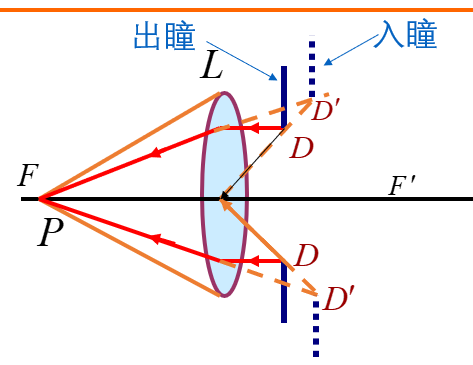
\includegraphics[width=8cm]{img/4.1.png}
            \end{figure}
入瞳是孔径光阑经过光阑后面的光学系统成的像,出瞳是经过前面的光学系统成的像。如果其在最前面,那本来就是入瞳,如果在最后面,本来就是出瞳。
\begin{description}[leftmargin=0.7cm,style=nextline,nosep]% nosep没有垂直间隔
    \item[物方孔径角] 轴上物点到入射光瞳 
\end{description}
\section{光学仪器}
\subsection{人眼}
\begin{itemize}
\item 
可见光的波长范围从400-760nm,人眼最灵敏的光波长为550nm。
\item  人眼瞳孔为\textbf{孔径光阑}
\end{itemize}
\begin{quote}
{\qquad\parindent2\ccwd\kaishu\zihao{5}
光照充足时对550nm最敏感;光照弱时对510nm敏感。
}
\end{quote}
\subsubsection{人眼的自动调节}
\begin{figure}[H]
    \centering
    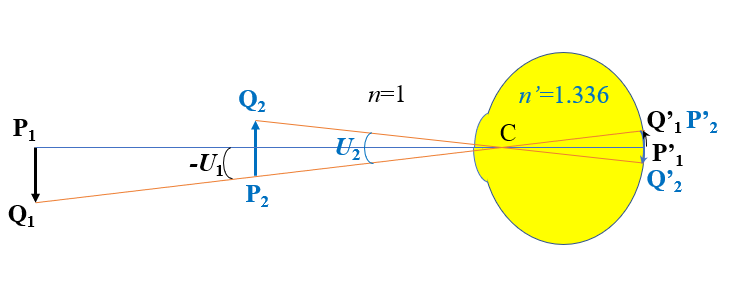
\includegraphics[width=7cm]{img/5.1.png}
    \end{figure}
\begin{description}[leftmargin=1.7cm,style=nextline,nosep]% nosep没有垂直间隔
    \item[远点] 眼睛调节到最远的距离,此时晶状体最薄,肌肉最松弛。
    \item[近点]   眼睛调节到最近的距离,此时晶状体最厚,肌肉最紧张。
    \item[远点距 r]  远点到眼睛物方主点的距离,注意$<0$
    \item[近点距 p ] ...
    \item[屈光度]  $R=1 /r ,P=1 /p ,A=R-P$
    \item[明视距离] $250mm$ 
    \item[视角]  人眼对物体的张角,遵从符号规则。 

\end{description}
\begin{equation}
\frac{1}{l_r}-\frac{1}{l_p}=R-P=A
\end{equation}

\subsubsection{非正常眼及其矫正}
        \begin{figure}[H]
            \centering
            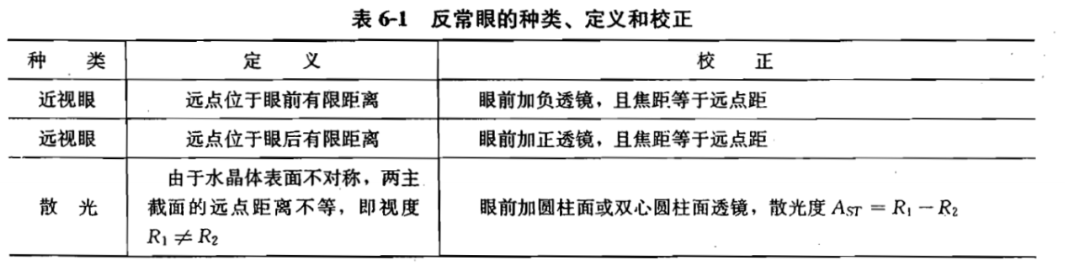
\includegraphics[width=7cm]{img/5.3.png}
            \end{figure}
\begin{quote}
{\qquad\parindent2\ccwd\kaishu\zihao{5}
1D 等于100 光焦度。对于正常眼,有$r=\infty,R=0,F'$ 在视网膜上。
}
\end{quote}
\begin{align*}
\Phi=\frac{1}{f'}=\frac{1}{l'}-\frac{1}{l}    
\end{align*}
对于所带光学系统而言,$l'=0.25$,l代入远点距。其实就是把无穷远处或者明视范围的物体成像到远点上。
\subsubsection{眼睛的自适应}
\begin{quote}
{\qquad\parindent2\ccwd\kaishu\zihao{5}
瞳孔直径改变
2~8mm

}
\end{quote}
\subsubsection{分辨本领}[]
\begin{definition}[极限分辨角]
    最靠近二点对人眼(物方节点)的张角$\phi$
\end{definition}
\begin{equation}
\phi=\frac{1.22 \lambda}{D(\text{入瞳直径})}\tag{6.1.2}
\end{equation}
一般取1度。

\section{放大镜}
视觉放大倍率,用\textbf{厘米}为单位。
\begin{equation}
    \Gamma =y_{i}^{\prime}/y_{e}^{\prime}=(l^{\prime}\tan \omega ^{\prime})/(l^{\prime}\tan \omega)= \tan \omega ^{\prime}/ \tan \omega  \tag{6.1.3}
\end{equation}

        \begin{figure}[H]
            \centering
            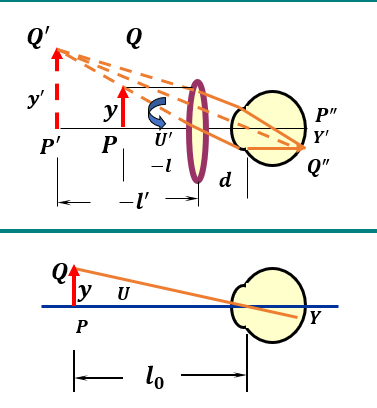
\includegraphics[width=7cm]{img/6.1.png}
            \end{figure}
\begin{equation}
\begin{aligned}
M_1&=\frac{\tan U'}{\tan U}=\frac{1}{\frac{y}{l_0}} \frac{y'}{-l'+d} \\
&=\frac{l_0}{y}\frac{y'}{d-l'}=\beta \frac{l_0}{d-l'}\\
&= \frac{l_0}{d-l'} -\frac{x'}{f'}=\frac{l_0}{f'} \frac{l'-f'}{l'-d} 
\end{aligned} \tag{6.1.4}
\end{equation}
$l'=-\infty$适合长时间观察,眼睛最放松.视角放大率与放大镜到眼睛距离无关.

如果在明视距离处,有
\begin{align}
   d-l'&=l_0 \tag{6.1.5.a}\\
   M&=-\frac{l'-f'}{f'}=\Phi  \tag{6.1.5.b} \\
   M&=\frac{f'-(d-l_0)}{f'}=\frac{l_0}{f'}+1-\frac{d}{f'} \tag{6.1.5.c}
\end{align}
当$d\to 0$ 
\begin{equation}
M_2=\frac{l_0}{f'}+1 \thickapprox M_2 \tag{6.1.6}
\end{equation}

\subsection{显微镜}
\begin{quote}
{\qquad\parindent2\ccwd\kaishu\zihao{5}
目:eye 物:obj。小物位于物镜焦点外侧,中间放大实像在$L_e$ 的物方焦面上,最后生成无限远或者明视距离放大的虚像。
}
\end{quote}
        \begin{figure}[H]
            \centering
            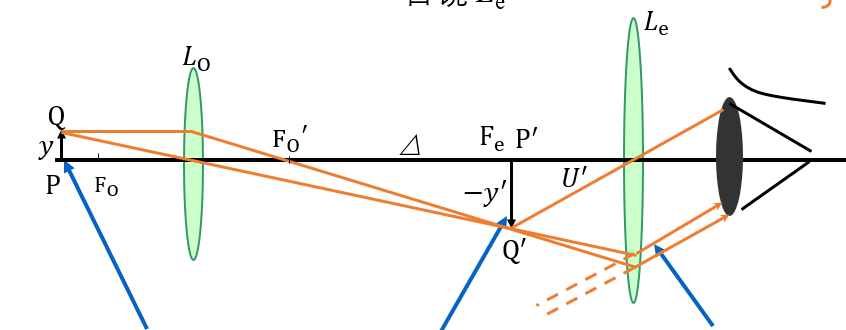
\includegraphics[width=8cm]{img/6.2.png}
            \caption*{注意看它的变量的表示}
            \end{figure}
最显然的,我们有
\begin{align}
    \Delta&=F'oF_e \tag{6.2.1.a} \\
     \tan U&=\frac{y}{l_0} \tag{6.2.1.b} \\
     \tan U'&=\frac{-y'}{f'_e}=--\frac{y'}{f'_e}=\frac{y'}{f'_e} \tag{6.2.1.c} \\
     M&=\frac{\tan U' }{\tan U}=\frac{l_0}{y}\frac{y'}{f'_e}=\beta_o M_e\tag{6.2.1.d}\\
     \beta_0&=-\frac{\Delta}{f_o'}\tag{6.2.1.e}\\     
     M&=-\frac{\Delta l_0}{f_o'f_e'}=\frac{l_0}{f'}\tag{6.2.1.f}
\end{align}
\subsection{望远镜}
        \begin{figure}[H]
            \centering
            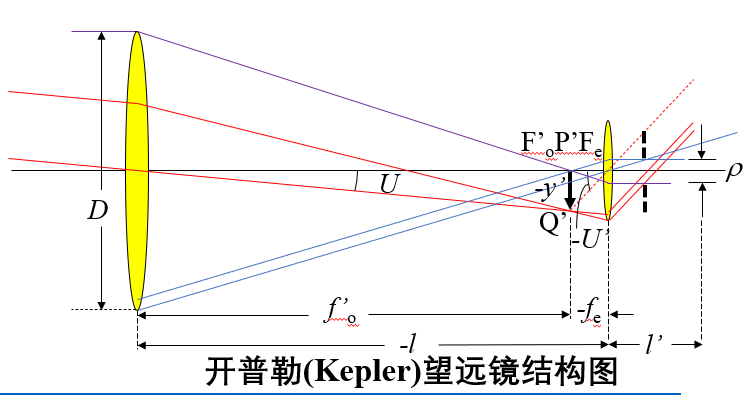
\includegraphics[width=8cm]{img/6.3.png}
            \end{figure}

\begin{quote}
{\qquad\parindent2\ccwd\kaishu\zihao{5}
观察无限远物体(天体)时望远镜的光学间隔为零,
观察有限远景物时望远镜的光学间隔很小。

}
\end{quote}
        \begin{figure}[H]
            \centering
            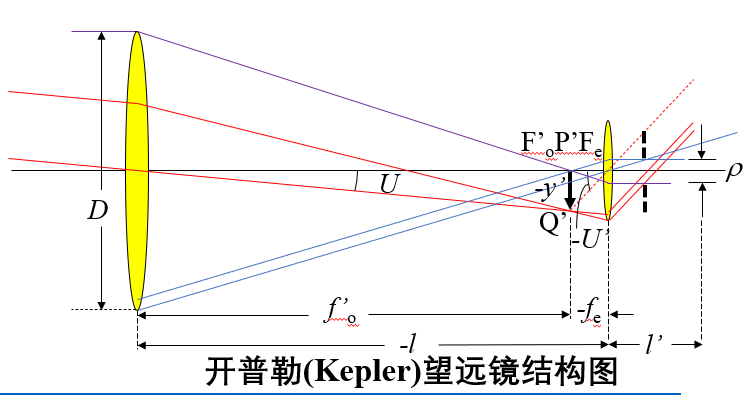
\includegraphics[width=7cm]{img/6.3.png}
            \end{figure}
该物体直接对眼镜成的像是
\begin{align}
\tan U&=\frac{-y'}{f'_o} \tag{6.3.1.a}\\
\tan -U'&=\frac{-y'}{-f'_e} \tag{6.3.1.b}\\
M&=\frac{\tan U'}{\tan U}=-\frac{f'_o}{f'_e}=-\frac{D}{\rho} \tag{6.3.1.c}
\end{align}
\begin{figure}[H]
    \centering
    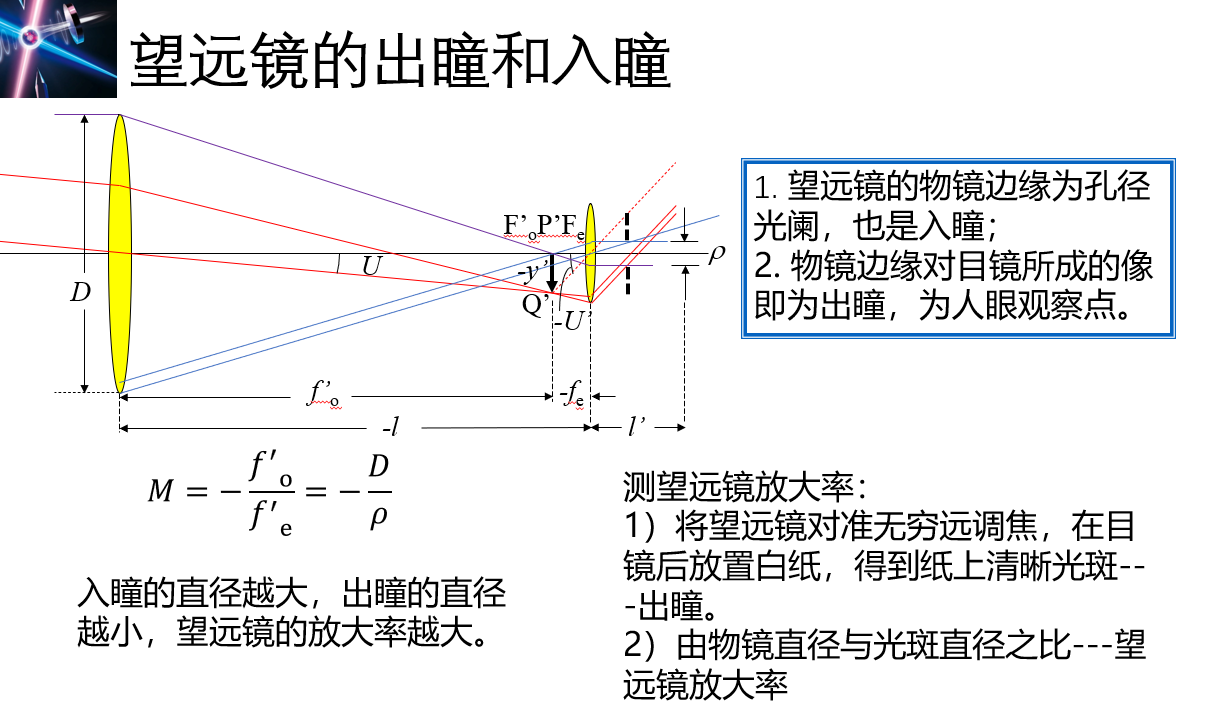
\includegraphics[width=7cm]{img/6.5.png}
    \end{figure}
\subsection{目镜}
目镜分为惠更斯(Huygens)目镜和冉斯登(Ramsten)目镜。
\subsection{照相机}
\subsection{投影仪}
\section{像差的种类和矫正}
        \begin{figure}[H]
            \centering
            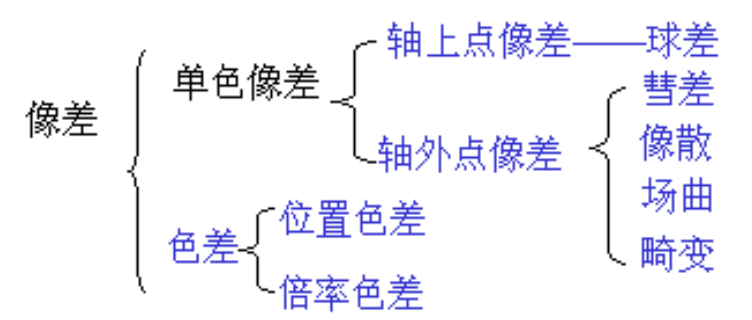
\includegraphics[width=7cm]{img/6.6.png}
            \end{figure}
\subsection{球差及其矫正}
球差是$\delta L=L'-l'$,正就是正球差,负就是负数球差。轴上,
\subsection{齐明点}
\begin{equation}
     nL=n'L=(n+n')r \tag{6.7.1}
\end{equation}
\begin{equation}
\beta=\frac{nL'}{n'L} \tag{6.7.2}
\end{equation}
三对齐明点另外的是
\begin{align}
 L&=L'=r \tag{6.7.3.a}\\
 L&=0   
\end{align}
\begin{quote}
{\qquad\parindent2\ccwd\kaishu\zihao{5}
注意上面的是像物距。
}
\subsubsection{等光程}
\end{quote}
\section{题目}
\begin{itemize}
\item 光程等于\textbf{介质中传播的几何路程何其折射率}的乘积
\item 基面一般是指(                    \textbf{ 焦平面、主平面和节平面}
)
理想光学系统不可能获得与立体物体相似的立体像是因为      ( \textbf{立体物体的轴向放大率和垂轴放大率是不等的
})
\item 注意明视距离         \begin{figure}[H]
            \centering
            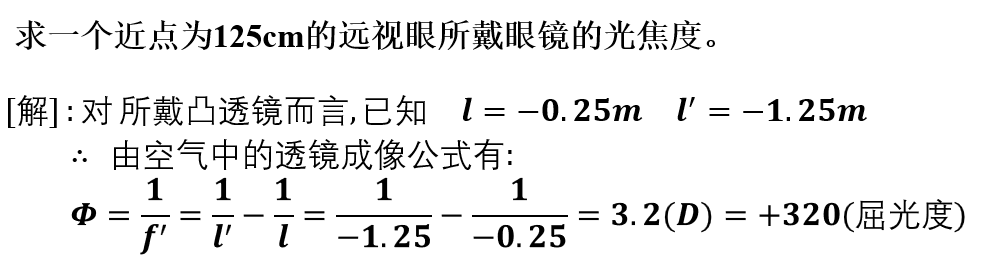
\includegraphics[width=8cm]{img/t1.png}
            \end{figure}
\end{itemize}